\documentclass[border=1pt]{standalone}
% Shared preamble for standalone figures in this directory.
% Compile with XeLaTeX from 讲义/figs, or via the figures target.
\usepackage{ctex}
\usepackage{amsmath}
\usepackage{amssymb}
\usepackage{bm}
\usepackage{mathtools}
\usepackage{tikz}
\renewcommand{\vec}[1]{\boldsymbol{#1}}
\newcommand{\cC}{\mathcal{C}}
\newcommand{\cD}{\mathcal{D}}
\newcommand{\R}{\mathbf{R}}
\usetikzlibrary{
    arrows.meta,
    calc,
    decorations.markings,
    angles,
    quotes,
    positioning,
    patterns,
    shapes.geometric
}

\begin{document}
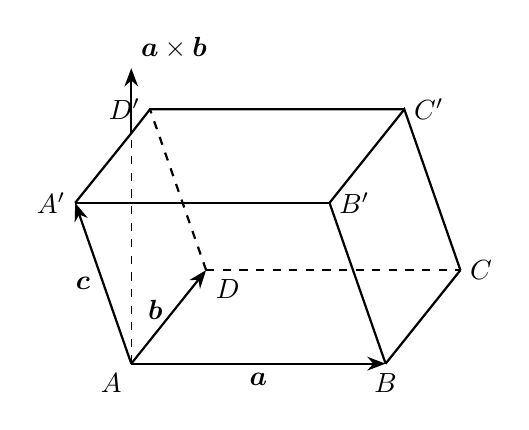
\begin{tikzpicture}[scale=0.95, >=Stealth]
    \coordinate (A) at (0,0);
    \coordinate (B) at (3.4,0);
    \coordinate (D) at (1.0,1.25);
    \coordinate (C) at (4.4,1.25);
    \coordinate (Ap) at (-0.75,2.15);
    \coordinate (Bp) at (2.65,2.15);
    \coordinate (Dp) at (0.25,3.40);
    \coordinate (Cp) at (3.65,3.40);
    \coordinate (H) at (0,3.08);
    \coordinate (N) at (0,3.95);

    \draw[->, thick] (A) -- (B);
    \draw[->, thick] (A) -- (D);
    \draw[thick] (B) -- (C);
    \draw[dashed, thick] (D) -- (C);

    \draw[->, thick] (A) -- (Ap);
    \draw[thick] (Ap) -- (Bp);
    \draw[thick] (B) -- (Bp);
    \draw[thick] (C) -- (Cp) -- (Bp);
    \draw[thick] (Ap) -- (H) -- (Dp) -- (Cp);
    \draw[dashed, thick] (D) -- (Dp);

    \draw[dashed] (A) -- (H);
    \draw[->, thick] (H) -- (N);

    \node[below left] at (A) {$A$};
    \node[below] at (B) {$B$};
    \node[right] at (C) {$C$};
    \node[below right] at (D) {$D$};
    \node[left] at (Ap) {$A'$};
    \node[right] at (Bp) {$B'$};
    \node[right] at (Cp) {$C'$};
    \node[left] at (Dp) {$D'$};

    \node[below] at (1.7,0) {$\vec{a}$};
    \node[left] at (0.55,0.72) {$\vec{b}$};
    \node[left] at (-0.42,1.08) {$\vec{c}$};
    \node[above right] at (N) {$\vec{a}\times\vec{b}$};
\end{tikzpicture}

\end{document}
